\id{МРНТИ 61.53.15}{https://doi.org/10.58805/kazutb.v.4.25-652}

\begin{articleheader}
\sectionwithauthors{Н.У. Нургалиев, Ж.Б. Искакова, А. Колпек, Е.К. Айбульдинов, А.С. Сабитов, Э.Е. Копишев, Т.Т. Машан, Л.А. Кусепова, Г.Ж. Алжанова, Г.Г. Абдиюсупов, М.Т. Өмірзақ}{СОВМЕСТНЫЙ ПИРОЛИЗ УГЛЯ И ВЫСОКОВЯЗКОЙ НЕФТИ}

{\bfseries \textsuperscript{1,2}Н.У.Нургалиев\textsuperscript{\envelope },
\textsuperscript{1}Ж.Б. Искакова\textsuperscript{\envelope },
\textsuperscript{3}А.Колпек, \textsuperscript{1}Е.К.
Айбульдинов\textsuperscript{\envelope },}

{\bfseries \textsuperscript{3}А.С.Сабитов , \textsuperscript{3}Э.Е.
Копишев, \textsuperscript{1,3}Т.Т. Машан, \textsuperscript{1,3}Л.А.
Кусепова, \textsuperscript{1}Г.Ж. Алжанова,}

{\bfseries \textsuperscript{1,4}Г.Г. Абдиюсупов, \textsuperscript{1,5}М.Т.
Өмірзақ}
\end{articleheader}

\begin{affiliation}
\textsuperscript{1}Научно-исследовательский институт Новых химических
технологий, Евразийский национальный университет им. Л.Н. Гумилева,
Астана, Казахстан,

\textsuperscript{2}Казахский университет технологии и бизнеса им. К.
Кулажанова, Астана, Казахстан,

\textsuperscript{3}Евразийский национальный университет им. Л.Н.
Гумилева, Астана, Казахстан,

\textsuperscript{4}CCS Services -- Central Asia, Алматы, Казахстан,

\textsuperscript{5}Sauda Exports\&Import, Алматы, Казахстан

\raggedright {\bfseries \textsuperscript{\envelope }} Корреспондент-автор:
\href{mailto:nurgaliev_nao@mail.ru}{\nolinkurl{nurgaliev\_nao@mail.ru}}
,
\href{mailto:zhanariskakova@mail.ru}{\nolinkurl{zhanariskakova@mail.ru}},
\href{mailto:elaman_@mail.ru}{\nolinkurl{elaman\_@mail.ru}}
\end{affiliation}

В статье предварительно проведен технический и элементный состав
исходного сырья (угля и высоковязкой нефти), а также определены
физико-химические показатели смолы сырья. Совместный пиролиз угля и
высоковязкой нефти осуществляли при различных добавках нефти в интервале
5-30 \%. Опыты проводили в алюминиевой реторте до 520 °С, в результате
которых получены такие продукты, как смола, пиролизный газ и полукокс.
При этом наибольший относительный прирост выходов смолы и пиролизного
газа наблюдался при добавке высоковязкой нефти, составляющей 20 \%, что
по всей видимости связано с наблюдаемым синэнергетическим эффектом,
основанном на взаимодействии угля и нефтяных фракций в процессе
термической обработки.

{\bfseries Ключевые слова:} уголь, высоковязкая нефть, совместный пиролиз,
смола, пиролизный газ, полукокс.

\begin{articleheader}
{\bfseries КӨМІР МЕН ТҰТҚЫРЛЫҒЫ ЖОҒАРЫ МҰНАЙДЫҢ БІРЛЕСКЕН ПИРОЛИЗІ}

{\bfseries \textsuperscript{1,2}Н.У.Нургалиев\textsuperscript{\envelope },
\textsuperscript{1}Ж.Б. Искакова\textsuperscript{\envelope },
\textsuperscript{3}А. Колпек, \textsuperscript{1}Е.К.
Айбульдинов\textsuperscript{\envelope },}

{\bfseries \textsuperscript{3}А.С. Сабитов, \textsuperscript{3}Э.Е. Копишев
, \textsuperscript{1,3}Т.Т. Машан, \textsuperscript{1,3}Л.А. Кусепова,
\textsuperscript{1}Г.Ж. Алжанова,}

{\bfseries \textsuperscript{1,4}Г.Г. Абдиюсупов, \textsuperscript{1,5}М.Т.
Өмірзақ}
\end{articleheader}

\begin{affiliation}
\textsuperscript{1}Жаңа химиялық технологиялар ғылыми-зерттеу институты,
Л.Н. Гумилев атындағы Еуразия ұлттық университеті, Астана, Қазақстан,

\textsuperscript{2}Қ.Құлажанов атындағы технология және бизнес
университеті, Астана, Қазақстан,

\textsuperscript{3}Л.Н. Гумилев атындағы Еуразия ұлттық университеті,
Астана, Қазақстан,

\textsuperscript{4}CCS Services -- Central Asia, Алматы, Қазақстан,

\textsuperscript{5}Sauda Exports\&Import, Алматы, Қазақстан,

e-mail:\href{mailto:nurgaliev_nao@mail.ru}{\nolinkurl{nurgaliev\_nao@mail.ru}}
,
\href{mailto:zhanariskakova@mail.ru}{\nolinkurl{zhanariskakova@mail.ru}},
\href{mailto:elaman_@mail.ru}{\nolinkurl{elaman\_@mail.ru}}
\end{affiliation}

Мақалада бастапқы шикізаттың (көмір және жоғары тұтқыр мұнай) техникалық
және элементтік құрамы алдын-ала жүргізіліп, шикізат шайырының
физика-химиялық көрсеткіштері анықталды. Көмір мен тұтқырлығы жоғары
мұнайдың бірлескен пиролизі әртүрлі мұнай қоспаларында 5-30\% аралығында
жүзеге асырылды. Тәжірибелер алюминий ретортында 520 °C-ге дейін
жүргізілді, нәтижесінде шайыр, пиролиз газы және жартылай кокс сияқты
өнімдер пайда болды. Сонымен қатар, мұнай мен пиролиз газының
шығымдылығының ең үлкен салыстырмалы өсімі жоғары тұтқыр мұнай
қоспасында байқалды, ол 20\%-ды құрайды, бұл термиялық өңдеу процесінде
көмір мен мұнай фракцияларының өзара әрекеттесуіне негізделген
синергетикалық әсерге байланысты.

{\bfseries Түйін сөздер:} көмір, тұтқырлығы жоғары мұнай, бірлескен
пиролиз, шайыр, пиролиз газы, жартылай кокс.

\begin{articleheader}
{\bfseries COMBINED PYROLYSIS OF COAL AND HIGH-VISCOSITY OIL}

{\bfseries \textsuperscript{1,2}N.U. Nurgaliyev\textsuperscript{\envelope },
\textsuperscript{1}Zh.B. Iskakova\textsuperscript{\envelope },
\textsuperscript{3}А. Kolpek, \textsuperscript{1}Ye.K.
Aibuldinov\textsuperscript{\envelope },}

{\bfseries \textsuperscript{3}A.S. Sabitov, \textsuperscript{3}E.Ye.
Kopishev, \textsuperscript{1,3}T.T. Mashan, \textsuperscript{1,3}L.A.
Kusepova, \textsuperscript{1}G.Zh. Alzhanova,\\
\textsuperscript{1,4}G.G. Abdiyussupov, \textsuperscript{1,5}М.Т.
Omirzak}
\end{articleheader}

\begin{affiliation}
\textsuperscript{1} Research Institute of New Chemical Technologies,
L.N. Gumilyov Eurasian National University, Astana, Kazakhstan,

\textsuperscript{2} Kazakh University of Technology and Business named
after K. Kulazhanov, Astana, Kazakhstan,

\textsuperscript{3} L.N. Gumilyov Eurasian National University, Astana,
Kazakhstan,

\textsuperscript{4}CCS Services -- Central Asia, Almaty, Kazakhstan,

\textsuperscript{5}Sauda Exports\&Import, Almaty, Kazakhstan

e-mail:
\href{mailto:nurgaliev_nao@mail.ru}{\nolinkurl{nurgaliev\_nao@mail.ru}}
,
\href{mailto:zhanariskakova@mail.ru}{\nolinkurl{zhanariskakova@mail.ru}},
\href{mailto:elaman_@mail.ru}{\nolinkurl{elaman\_@mail.ru}}
\end{affiliation}

In the article provides a preliminary technical and elemental
composition of the feedstock (coal and high-viscosity oil), and also
determines the physicochemical properties of the resin of the feedstock.
Coal and high-viscosity oil were combined pyrolysis with various oil
additives in the range of 5-30\%. The experiments were carried out in an
aluminum retort at temperatures up to 520 °C, resulting in the following
products: tar, pyrolysis gas, and semi-coke. The greatest relative
increase in oil and pyrolysis gas yields was observed with the addition
of high-viscosity oil, amounting to 20\%, which is apparently due to the
observed synergy effect based on the interaction of coal and oil
fractions during heat treatment.

{\bfseries Keywords:} coal, high-viscosity oil, combined pyrolysis, tar,
pyrolysis gas, semi-coke.

\begin{multicols}{2}
{\bfseries Введение.} Во многих странах (Казахстан, Китай и др.) запасы
угля значительно больше, чем запасы нефти и природного газа. Все больший
интерес в настоящее время привлекают исследования по совместному
пиролизу угля и высоковязкой нефти, биомассы, горючего сланца, отходов
полимерных пластиков и других органических материалов. Исследования в
основном сосредоточены на двух аспектах. Один из них ̶ это оптимизация
выхода смолы и компонента, а другой ̶ учет синергетического эффекта при
пиролизе. Например, при совместном пиролизе биомассы было обнаружено,
что такой подход улучшает не только выход и свойства смолы, но и
теплотворную способность кокса, смолы и газа {[}1{]}.

Характеристики пиролиза угольного топлива и нефтяного шлама и были
изучены с помощью термогравиметрического анализатора в атмосфере аргона
{[}2{]}. В исследовании {[}3{]} основное внимание уделяется
потенциальному использованию горючего сланца в качестве сырья для
коксования угольной смеси, а также предлагается сопиролиз различных
марок углей со сланцем с точки зрения коксования угольной смеси.
Добавление низкосортного угля к сланцу может повысить выход смолы и
увеличить содержание газов CO, CH\textsubscript{4} и H\textsubscript{2}
при микроволновом нагреве {[}4{]}. Кроме того, при пиролизе
низкосортного угля и пластика выход кокса снижается, а выход смолы
повышается с увеличением доли пластиковой добавки {[}5{]}. Результаты
исследования микроволнового сопиролиза угля и биомассы показали, что
микроволновый абсорбер может косвенно нагревать частицы угля и биомассы,
которые относительно прозрачны для микроволн и влияют на выход и
качество продукта, выступая в качестве каталитических прекурсоров
{[}6{]}. Синергетический эффект от совместного пиролиза низкосортного
угля и биомассы становится все более значительным по мере уменьшения
марки угля, возможно, потому, что исходная структура этих углей содержит
крупные поры и небольшие кластеры ароматических структур, которые легко
сохраняются в виде смолы при быстром сопиролизе {[}7{]}. При
исследовании характеристик сопиролиза угля и сельскохозяйственных
отходов было обнаружено, что соотношение смешивания является основным
фактором, влияющим на выход и состав смолы и газа, а синергетический
эффект значителен во время пиролиза угля и биомассы, но минимален во
время совместного пиролиза {[}8{]}. При изучении характеристик
сопиролиза различных марок угля и горючего сланца обнаружена синергия в
ходе процесса, при этом уголь обеспечивает водород для горючего сланца,
что увеличивает выход смолы и служит компонентом смолы с высокой
добавленной стоимостью {[}9{]}. Совместный пиролиз опилок и
битуминозного угля (в различных соотношениях смешивания и температурах)
улучшает выход газа, но снижает выход смолы {[}10{]}. Авторы в работе
{[}11{]} обобщили результаты исследований по сопиролизу угля и отходов,
таких как плавающие в сточных водах водоросли, солома, отходы пластика,
отходы смазочного масла, отходы минерального масла и горючий сланец.
Авторы предложили использовать синергетические эффекты в зависимости от
различных целевых продуктов для добавления соответствующих отходов и
улучшения выхода газа, кокса и смолы, а также качества продуктов.

Таким образом, типы и свойства используемых добавок влияют на пиролиз
угля. Добавки перераспределяют и модифицируют продукты пиролиза.
Например, тяжелая смола преобразуется в легкую смолу, или выход газа с
высокой теплотворной способностью увеличивается или уменьшается.

Такое углеводородное сырье как тяжелая (высоковязкая) нефть с высокой
плотностью и сложным составом в основном используется в качестве мазута
{[}12{]}. Обычно такая нефть имеет повышенную влажность и вязкость, что
связано с повышенным содержанием в их составе смоли­сто-асфальтеновых
веществ. Нефтеперерабатывающие заводы не способны перерабатывать
высоковязкие нефти по стандартным схемам {[}13{]}. Однако по мере
повышения температуры тяжелая нефть может свободно перетекать во влажные
частицы угля полностью из-за повышенной текучести тяжелой нефти во время
совместного пиролиза с углем. Уголь и тяжелая нефть могут полностью
реагировать во время пиролиза, чтобы получить продукты с высокой
добавленной стоимостью. Этот эффект достигается за счет того, что
тяжелая нефть не только связывает частицы угля вместе, но и значительно
увеличивает площадь контакта угля и тяжелой нефти. В связи с этим, целью
данной работы является исследование влияния добавок высоковязкой нефти
на выход продуктов совместного пиролиза (смола, пиролизный газ и
полукокс).

{\bfseries Материалы и методы.} В качестве сырья для совместного пиролиза
выбраны уголь месторождения «Сарыадыр» и высоковязкая нефть
месторождения «Зайсан».

Для определения влажности, зольности, летучих веществ, серы, выходов
продуктов полукоксования, плотности, элементного состава и др.,
использовали методы в соответствии с ГОСТ 11014-2001, ГОСТ 11022-95 (ISO
1171-97), ГОСТ 1437-75, ГОСТ 3168-93, ГОСТ 1437-75 , ГОСТ 6382-2001,
ГОСТ 10538-87, ГОСТ 8606-93 (ISO 334-92), ASTM D 5291 (Standard Test
Methods for Instrumental Determination of Carbon, Hydrogen, and Nitrogen
in Petroleum Products and Lubricants).

Пиролиз проводили в алюминиевой реторте до 520 °С в соответствии с
методикой, описанной в работе {[}14{]}. Пиролиз осуществляли при
различных добавках нефти (5, 10, 15, 20, 25, 30 \%) при массовых
соотношениях угля и нефти соответственно 95/5, 90/10, 85/15, 80/20,
75/25, 70/30.

{\bfseries Результаты и обсуждение.} Для сравнения в таблице 1 приведены
результаты элементного и технического анализа исходного сырья ̶ угля и
нефти. Как видно, высоковязкая нефть обладает очень низкой зольностью и
существенно более высокими значениями выходов летучих веществ и
содержания углерода и водорода по сравнению с углем.

Результаты физико-химических показателей смолы угля и высоковязкой
нефти, представленных в таблице 2, показали, что во фракционном составе
как смолы угля, так и смолы нефти присутствуют в основном среднекипящие
и высококипящие фракции. Причем в смоле нефти преобладают среднекипящие
фракции (44,1 \%), которые содержат множество важных компонентов
(комплексные смеси), таких как ароматические углеводороды, смолы,
циклические и оксигенсодержащие соединения, являющиеся ключевыми для
производства бензина и других моторных топлив. Вместе с тем, в смоле
угля преобладают высококипящие фракции (47,4 \%), содержащие более
тяжелые соединения, такие как асфальты, вакуумные дистилляты, парафины и
цинковые соединения, коксы. Сравнительный анализ группового состава угля
и нефти показал, что в смоле угля содержатся больше ароматических
углеводородов и гетероатомных соединений, чем в смоле нефти, в которой,
в свою очередь, преобладают парафины и изо-парафины и нафтены.
\end{multicols}

\begin{table}[H]
\caption*{Таблица 1 ̶ Характеристики исходного сырья}
\centering
\begin{tabular}{|l|rr|}
\hline
\multirow{2}{*}{Параметр, \%}           & \multicolumn{2}{l|}{Вид сырья}                                       \\ \cline{2-3} 
                                        & \multicolumn{1}{l|}{Уголь} & \multicolumn{1}{l|}{Высоковязкая нефть} \\ \hline
Влажность на рабочую массу, Wtr         & \multicolumn{1}{r|}{6,4}   & 6,5                                     \\ \hline
Зольность на сухую массу, Ad            & \multicolumn{1}{r|}{31,31} & 0,1                                     \\ \hline
Выход летучих и связанный углерод кокса & \multicolumn{1}{r|}{30,1}  & 93,4                                    \\ \hline
Элементный состав на сухую массу:       & \multicolumn{1}{l|}{}      & \multicolumn{1}{l|}{}                   \\ \hline
C                                       & \multicolumn{1}{r|}{58,3}  & 81,6                                    \\ \hline
H                                       & \multicolumn{1}{r|}{5,6}   & 10,1                                    \\ \hline
N                                       & \multicolumn{1}{r|}{1}     & 0,5                                     \\ \hline
O                                       & \multicolumn{1}{r|}{3}     & 6,1                                     \\ \hline
S                                       & \multicolumn{1}{r|}{0,5}   & 1,7                                     \\ \hline
\end{tabular}
\end{table}

\begin{table}[H]
\caption*{Таблица 2 - Физико-химические показатели смолы угля и
высоковязкой нефти}
\centering
\begin{tabular}{|l|r|r|}
\hline
                           & \multicolumn{1}{l|}{Уголь} & \multicolumn{1}{l|}{Высоковязкая нефть} \\ \hline
Плотность, т/м$^3$            & 0,935                      & 0,994                                   \\ \hline
Фракционный состав, \%:    & \multicolumn{1}{l|}{}      & \multicolumn{1}{l|}{}                   \\ \hline
нк – 200 $^o$С                & 13,2                       & 19,1                                    \\ \hline
200 – 360 $^o$С               & 39,4                       & 44,1                                    \\ \hline
\textgreater{}360 $^o$С       & 47,4                       & 36,8                                    \\ \hline
Групповой состав, \%:      & \multicolumn{1}{l|}{}      & \multicolumn{1}{l|}{}                   \\ \hline
Парафины и изо-парафины    & 26,7                       & 38,3                                    \\ \hline
Олефины и циклоолефины     & 10,3                       & 12,4                                    \\ \hline
Нафтены                    & 3,5                        & 17,2                                    \\ \hline
Ароматические углеводороды & 32,1                       & 22,6                                    \\ \hline
Гетероатомные соединения   & 27,4                       & 9,5                                     \\ \hline
\end{tabular}
\end{table}

\begin{table}[H]
\caption*{Таблица 3 - Результаты процесса совместного пиролиза угля и
нефти}
\centering
\begin{tabular}{|r|l|r|r|r|r|}
\hline
\multicolumn{1}{|l|}{№} &
  Образец &
  \multicolumn{1}{l|}{Влага, War, \%} &
  \multicolumn{1}{l|}{Смола, \%} &
  \multicolumn{1}{p{0.21\textwidth}|}{Полукокс, (крекинг-остаток) \%} &
  \multicolumn{1}{l|}{Газ, \%} \\ \hline
1 & Уголь                    & 6,4 & 5,1  & 84,8 & 3,7  \\ \hline
2 & Высоковязкая нефть (ВВН) & 6,5 & 74,9 & 7,2  & 11,4 \\ \hline
3 & Уголь/ВВН (95/5)         & 6,4 & 9,2  & 79,1 & 4,3  \\ \hline
4 & Уголь /ВВН (90/10)       & 6,4 & 12,1 & 76,4 & 4,6  \\ \hline
5 & Уголь/ВВН(85/15)         & 6,4 & 15   & 72,5 & 5    \\ \hline
6 & Уголь/ВВН(80/20)         & 6,4 & 20,4 & 65,9 & 5,5  \\ \hline
7 & Уголь/ВВН(75/25)         & 6,4 & 23,1 & 62,4 & 5,9  \\ \hline
8 & Уголь/ВВН(70/30)         & 6,4 & 25,3 & 59,1 & 6,2  \\ \hline
\end{tabular}
\end{table}

\begin{multicols}{2}
\emph{Выход продуктов совместного пиролиза} \emph{угля и нефти} (смола,
пиролизный газ, полукокс). Результаты проведения процесса совместного
пиролиза угля и высоковязкой нефти приведены в таблице 3 и на рисунке 1.
Добавление высоковязкой нефти к углю от 5 до 30 \% приводит к
благоприятному протеканию совместного пиролиза, что отражается на
существенном повышении выхода смолы с 5,1 до 25,3 \%, вследствие того,
что нефть характеризуется повышенным содержанием смолисто-асфальтеновых
веществ. Также наблюдается постепенное увеличение пиролизного газа с 3,7
до 6,2 \%, а содержание полукокса значительно снижается с 84,8 до 59,1
\%. Аналогичный эффект от добавки высоковязкой нефти к углю в процессе
их совместного пиролиза наблюдается в работе {[}15{]}, в которой выход
кокса снизился на 20\%, а выход газа и смолы увеличился на 7,74 и
12,18\%. При этом количество гидроксильных групп на поверхности кокса
уменьшилось, а содержание алканов и фенолов в смоле снизилось на 7,89 и
8,10\%, соответственно. Содержание ароматических веществ увеличилось на
21,60 \%. Содержание CO\textsubscript{2}, CH\textsubscript{4} и
C\textsubscript{n}H\textsubscript{m} увеличилось примерно в два раза по
сравнению с исходным количеством, тогда как содержание CO и
H\textsubscript{2} уменьшилось на 2,88 и 22,18\% соответственно.
\end{multicols}

\begin{figure}[H]
	\centering
	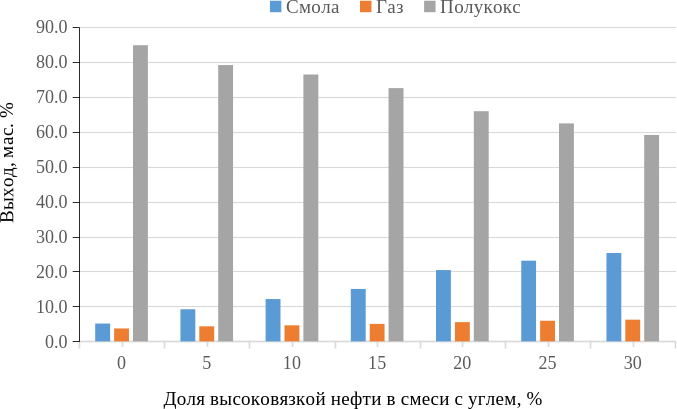
\includegraphics[width=0.8\textwidth]{media/chem/image113}
	\caption*{Рис. 1 - Влияние различных добавок высоковязкой нефти к
совместному пиролизу с углем}
\end{figure}

\begin{multicols}{2}
На рисунках 2 и 3 приведен относительный прирост выходов смолы и
пиролизного газа (V=(V\textsubscript{i+1 ̶}
V\textsubscript{i})/V\textsubscript{i}) при добавках в интервале 10-30
\%, откуда видно, что наибольший прирост выхода наблюдается при добавке
высоковязкой нефти, составляющей 20 \%. Это можно объяснить наблюдаемым
синэнергетическим эффектом, основанном на взаимодействии угля и нефтяных
фракций в процессе термической обработки. Механизм этого эффекта можно
рассмотреть по нескольким ключевым аспектам: 1)повышение температуры
пиролиза и ускорение реакций (высоковязкая нефть содержит углеводороды,
которые при нагревании могут выделять дополнительную энергию и повышать
температуру в реакционной зоне, что способствует ускорению
термохимических реакций); 2)коагуляция и улучшение теплопередачи (нефть
может образовывать тонкие пленки на поверхности угольных частиц, что
улучшает теплопередачу, а это помогает избежать перегрева отдельных
участков и способствует более равномерному распределению тепла и
разложению угля); 3)каталитическое действие (некоторые компоненты
высоковязкой нефти могут играть роль катализаторов, ускоряя реакции
пиролиза и способствуя более полному разложению угля, что повышает выход
ценных продуктов); 4)снижение образования коксующихся остатков (это
улучшает выход и качество конечных продуктов пиролиза и снижает
проблемы, связанные с образованием кокса. Таким образом,
синэнергетический эффект позволяет повысить эффективность пиролиза угля,
улучшить выход ценных продуктов и снизить отрицательные последствия,
связанные с образованием коксующихся остатков.
\end{multicols}


\begin{figure}[H]
	\centering
	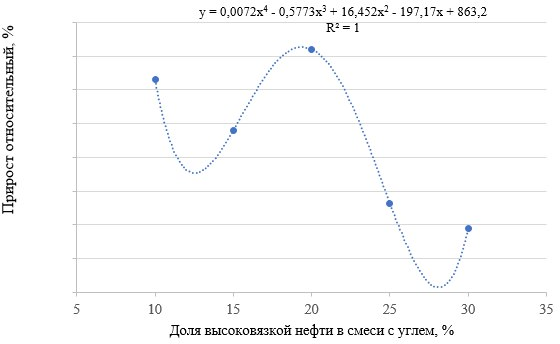
\includegraphics[width=0.8\textwidth]{media/chem/image114}
	\caption*{Рис. 2 - Влияние высоковязкой нефти на относительный прирост
выхода смолы}
\end{figure}

\begin{figure}[H]
	\centering
	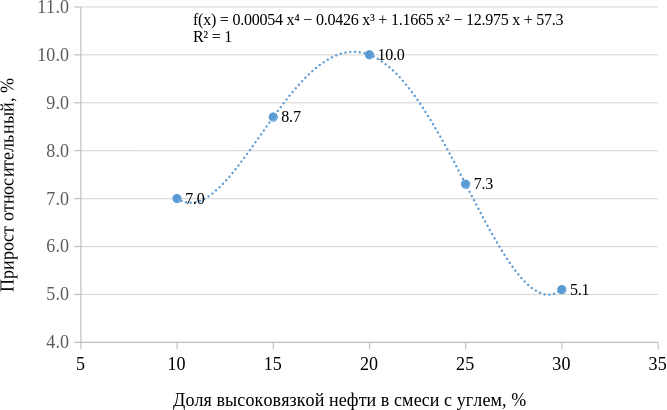
\includegraphics[width=0.8\textwidth]{media/chem/image115}
	\caption*{Рис. 3 ̶ Влияние высоковязкой нефти на относительный прирост
выхода пиролизного газа}
\end{figure}

\begin{multicols}{2}
{\bfseries Выводы.} Результаты данной работы продемонстрировали реализацию
возможности совместного пиролиза угля и высоковязкой нефти. Добавки
последней приводят к небольшому увеличению пиролизного газа и
существенному повышению смолы, за счет в основном высокого содержания
смол и асфальтенов в высоковязкой нефти. Также наблюдается значительное
снижение полукокса. Добавка высоковязкой нефти к углю в количестве 20 \%
приводит к максимальному относительному приросту выходов смолы и
пиролизного газа, что может быть связано с синэнергетическим эффектом,
который основан на взаимодействии угля и нефтяных фракций в процессе их
термической деструкции. Таким образом, несмотря на большие трудности
переработки высоковязкой нефти по стандартным методам, возможным
решением проблемы вовлечения такой нефти в топливно-энергетический и
нефтехимический баланс может быть проведение совместного пиролиза
высоковязкой нефти с подходящим (по физико-химическим характеристикам)
сырьем. Таким образом, совместный пиролиз угля и высоковязкой нефти
может быть перспективным направлением и значительным потенциалом для
создания эффективных и экологически чистых технологий в области
переработки углеводородных ресурсов. Данная методология может
способствовать улучшению качественных характеристик продуктов, а также
повышению общей эффективности процесса.

\emph{{\bfseries Финансирование.}Настоящая работа выполнена при финансовой
поддержке Комитета науки Министерства науки и высшего образования
Республики Казахстан (№ BR21882171 «ЦУР 9.4: Развитие «зеленой»
экономики Казахстана путем переработки минерального сырья и отходов
методом пиролиза»).}
\end{multicols}

\begin{center}
{\bfseries Литература}
\end{center}

\begin{references}
1. Abnisa, F.; Wan Daud, W. M. A. A review on co-pyrolysis of biomass:
An optional technique to obtain high-grade pyrolysis oil // Energy
Convers. Manage, 2014.- Vol.87.- Р.71-85.

DOI 10.1016/j.enconman.2014.07.007

2. Xiaoyu Li, Xiaoxi Yang, Gang Cheng, Hongqing Feng, Xiaojie Liu,
Yufeng Ma. Experimental study on co-pyrolysis of oil sludge and coal //
Advanced Materials Research, 2012.- Vol. 356-360.- P. 2515-2519. DOI
10.4028/www.scientific.net/AMR.356-360.2515

3. Xiangchun Liu, Ping Cui, Qiang Ling, Zhigang Zhao, Ruilun Xie. A
review on co-pyrolysis of coal and oil shale to produce coke //
\href{https://link.springer.com/journal/11705}{Frontiers of Chemical
Science and Engineering}.- 2020.-Vol.~14.- P. 504 - 512.
\href{https://doi.org/10.1007/s11705-019-1850-z}{DOI
10.1007/s11705-019-1850-z}

4. Song, Y.-h.; She, J.-m.; Lan, X.-z.; et al. Pyrolysis of Low
Metamorphic Coal and Oil Shale by Microwave Irradiation // Coal Convers,
2012.- Vol.35 (2).- P. 22-26.

5. Lan, X.-z., Liu, Q.-n., Song, Y.-h. Study on co-pyrolysis of low
metamorphic coal and plastic with microwave // Coal Convers.- 2012. -
Vol. 35(1).- P. 16-19.

6. Mushtaq F., Mat R., Ani F. N. A review on microwave assisted
pyrolysis of coal and biomass for fuel production // Renewable
Sustainable Energy Rev.- 2014. - Vol. 39.- P.555-574.

DOI 10.1016/j.rser.2014.07.073

7. Soncini R. M., Means N.C., Weiland N.T. Co-pyrolysis of low rank
coals and biomass: Product \\distributions // Fuel.- 2013. -Vol. 112.- P.
74-82. DOI 10.1016/j.fuel.2013.04.073

8. Aboyade A.O., Carrier M., Meyer E.L.,Knoetze H., Görgens J.F. Slow
and pressurized co-pyrolysis of coal and agricultural residues // Energy
Convers. Manage.- 2013. - Vol. 65.- P. 198-207. DOI
\\10.1016/j.enconman.2012.08.006

9. Miao Z.-y., Wu G.-g., Li P., Meng X.-l., Zheng Z.-l. Investigation
into co-pyrolysis characteristics of oil shale and coal // Int. J. Min.
Sci. Technol. -2012. - Vol. 22.- P. 245-249.

DOI 10.1016/j.ijmst.2011.09.003

10. Liang P., Han Z.-h., Wu J.-f., Zhang R., Bi J. Research on
synergetic reactivity of bituminous coal and saw dust during copyrolysis
in a fixed bed // J. Chem. Ind. Eng.- 2014. - Vol. 35 (1).- P. 1-5.

11. He X.-m., Wang C.-x., Fu P.-r., et al. Survey of Co-pyrolysis of
Rank Coal and Waste // Energy Environ. Prot.- 2014. - Vol. 28 (1). - P.
25-29.

12. Zhang J.-m., Liu G. Comprehensive Utilization of Low-Temperature
Coal Tar // Coal Convers.- 2010. - Vol. 33(3).- P. 92-96.

13. Тухватуллина А.З., Кемалов А.Ф., Кемалов Р.А., Юсупова Т.Н. Анализ
состава и свойств высоковязких нефти и их влияние на процессы коксования
// Материалы Международной научно-практической конференции «Высоковязкие
нефти и природные битумы: проблемы повышения эффективности разведки и
разработки месторождений», Казань.- 2012.-С. 314-316.

14. Нургалиев Н.У., Искакова Ж.Б., Колпек А., Айбульдинов Е.К., Сабитов
А.С., Копишев Э.Е., Салихов Р.М., Петров М.С., Алжанова Г.Ж., Абдиюсупов
Г.Г., Өмірзақ М.Т. Исследование физико-химических характеристик угля и
продуктов его пиролиза // Вестник КазУТБ, 2024. - №3 (24). - С.277-287.
DOI 10.58805/kazutb.v.3.24-470.

15. Yong-hui Song, Qiao-na Ma, Wen-jin He. Co-pyrolysis Properties and
Product Composition of Low-Rank Coal and Heavy Oil // Energy \& Fuels,
2016. - Vol. 31(1). -- Р. 217--223. DOI
\\10.1021/acs.energyfuels.6b02106.
\end{references}

\begin{center}
{\bfseries References}
\end{center}

\begin{references}
1. Abnisa, F.; Wan Daud, W. M. A. A review on co-pyrolysis of biomass:
An optional technique to obtain high-grade pyrolysis oil // Energy
Convers. Manage, 2014.- Vol.87.- Р.71-85.

DOI 10.1016/j.enconman.2014.07.007

2. Xiaoyu Li, Xiaoxi Yang, Gang Cheng, Hongqing Feng, Xiaojie Liu,
Yufeng Ma. Experimental study on co-pyrolysis of oil sludge and coal //
Advanced Materials Research, 2012.- Vol. 356-360.- P. 2515-2519. DOI
10.4028/www.scientific.net/AMR.356-360.2515

3. Xiangchun Liu, Ping Cui, Qiang Ling, Zhigang Zhao, Ruilun Xie. A
review on co-pyrolysis of coal and oil shale to produce coke //
\href{https://link.springer.com/journal/11705}{Frontiers of Chemical
Science and Engineering}.- 2020.-Vol.~14.- P. 504 - 512.
\href{https://doi.org/10.1007/s11705-019-1850-z}{DOI
10.1007/s11705-019-1850-z}

4. Song, Y.-h.; She, J.-m.; Lan, X.-z.; et al. Pyrolysis of Low
Metamorphic Coal and Oil Shale by Microwave Irradiation // Coal Convers,
2012.- Vol.35 (2).- P. 22-26.

5. Lan, X.-z., Liu, Q.-n., Song, Y.-h. Study on co-pyrolysis of low
metamorphic coal and plastic with microwave // Coal Convers.- 2012. -
Vol. 35(1).- P. 16-19.

6. Mushtaq F., Mat R., Ani F. N. A review on microwave assisted
pyrolysis of coal and biomass for fuel production // Renewable
Sustainable Energy Rev.- 2014. - Vol. 39.- P.555-574.

DOI 10.1016/j.rser.2014.07.073

7. Soncini R. M., Means N.C., Weiland N.T. Co-pyrolysis of low rank
coals and biomass: Product \\distributions // Fuel.- 2013. -Vol. 112.- P.
74-82. DOI 10.1016/j.fuel.2013.04.073

8. Aboyade A.O., Carrier M., Meyer E.L.,Knoetze H., Görgens J.F. Slow
and pressurized co-pyrolysis of coal and agricultural residues // Energy
Convers. Manage.- 2013. - Vol. 65.- P. 198-207. DOI
\\10.1016/j.enconman.2012.08.006

9. Miao Z.-y., Wu G.-g., Li P., Meng X.-l., Zheng Z.-l. Investigation
into co-pyrolysis characteristics of oil shale and coal // Int. J. Min.
Sci. Technol. -2012. - Vol. 22.- P. 245-249.

DOI 10.1016/j.ijmst.2011.09.003

10. Liang P., Han Z.-h., Wu J.-f., Zhang R., Bi J. Research on
synergetic reactivity of bituminous coal and saw dust during copyrolysis
in a fixed bed // J. Chem. Ind. Eng.- 2014. - Vol. 35 (1).- P. 1-5.

11. He X.-m., Wang C.-x., Fu P.-r., et al. Survey of Co-pyrolysis of
Rank Coal and Waste // Energy Environ. Prot.- 2014. - Vol. 28 (1). - P.
25-29.

12. Zhang J.-m., Liu G. Comprehensive Utilization of Low-Temperature
Coal Tar // Coal Convers.- 2010. - Vol. 33(3).- P. 92-96.

13. Tuhvatullina A.Z., Kemalov A.F., Kemalov R.A., Jusupova T.N. Analiz
sostava i svojstv vysokovjazkih nefti i ih vlijanie na processy
koksovanija // Materialy Mezhdunarodnoj nauchno-prakticheskoj
konferencii «Vysokovjazkie nefti i prirodnye bitumy: problemy
povyshenija jeffektivnosti razvedki i razrabotki\\ mestorozhdenij»,
Kazan'.- 2012.-S. 314-316.{[}in Russian{]}

14. Nurgaliev N.U., Iskakova Zh.B., Kolpek A.,
Ajbul' dinov E.K., Sabitov A.S., Kopishev Je.E., Salihov
R.M., Petrov M.S., Alzhanova G.Zh., Abdijusupov G.G., Өmіrzaқ M.T.
Issledovanie fiziko-himicheskih harakteristik uglja i produktov ego
piroliza // Vestnik KazUTB, 2024. - №3 (24). - S.277-287. DOI
\\10.58805/kazutb.v.3.24-470. {[}in Russian{]}

15. Yong-hui Song, Qiao-na Ma, Wen-jin He. Co-pyrolysis Properties and
Product Composition of Low-Rank Coal and Heavy Oil // Energy \& Fuels,
2016. - Vol. 31(1). -- Р. 217--223. \\DOI 10.1021/acs.energyfuels.6b02106
\end{references}

\begin{authorinfo}
\hspace{1em}\emph{{\bfseries Сведения об авторах}}

Нургалиев Н.У.-кандидат химических наук, ассоциированный профессор,
;Казахский университет технологии и бизнеса имени К.Кулажанова, Астана
Казахстан, e-mail:
\href{mailto:nurgaliev_nao@mail.ru}{\nolinkurl{nurgaliev\_nao@mail.ru}};

Искакова Ж.Б.- кандидат химических наук, ассоциированный профессор
(доцент), Научно-исследовательский институт Новых химических технологий,
Евразийский национальный университет им. Л.Н. Гумилева, Астана,
Казахстан, e-mail:
\href{mailto:zhanariskakova@mail.ru}{\nolinkurl{zhanariskakova@mail.ru}};

Колпек А.- кандидат химических наук, ассоциированный профессор (доцент),
Евразийский национальный университет им. Л.Н. Гумилева, Астана,
Казахстан,e-mail:
\href{mailto:aynagulk@mail.ru}{\nolinkurl{aynagulk@mail.ru}};

Айбульдинов Е.К.-доктор PhD, Научно-исследовательский институт Новых
химических технологий, Евразийский национальный университет им. Л.Н.
Гумилева, Астана,Казахстан, e-mail:
\href{mailto:elaman_@mail.ru}{\nolinkurl{elaman\_@mail.ru}};

Сабитов А.С.- докторант, Евразийский национальный университет им. Л.Н.
Гумилева, Астана, Казахстан, e-mail:
\\\href{mailto:sawy552@gmail.com}{\nolinkurl{sawy552@gmail.com}};

Копишев Э.Е.-кандидат химических наук, Евразийский национальный
университет им. Л.Н. Гумилева, Астана, Казахстан, e-mail:
\href{mailto:eldar_kopishev@mail.ru}{\nolinkurl{eldar\_kopishev@mail.ru}};

Машан Т.Т.- кандидат химических наук, доцент, Евразийский национальный
университет им. Л.Н.Гумилева, Астана, Казахстан, e-mail:
togzhan-mashan@mail.ru;

Кусепова Л.А.-кандидат химических наук, доцент, Евразийский национальный
университет им. Л.Н. Гумилева, Астана, Казахстан, e-mail:
kusepova71@mail.ru;

Алжанова Г.Ж.-докторант, Научно-исследовательский институт Новых
химических технологий, Евразийский национальный университет им. Л.Н.
Гумилева, Астана, Казахстан, e-mail:
\href{mailto:galiya.alzhanova@gmail.com}{\nolinkurl{galiya.alzhanova@gmail.com}};

Абдиюсупов Г.Г.-менеджер, ТОО «CCS Services -- Central Asia»,Астана,
Казахстан, e-mail:
\href{mailto:gaziz_86@inbox.ru}{\nolinkurl{gaziz\_86@inbox.ru}};

Өмірзақ М.Т.- доктор PhD, ТОО «Sauda Exports\&Import», Астана
Казахстан,e-mail:
\href{mailto:madi.omirzak@gmail.com}{\nolinkurl{madi.omirzak@gmail.com}}

\hspace{1em}\emph{{\bfseries Information about the authors}}

Nurgaliyev N.U.- Candidate of Chemical Science, Associate Professor, ,
Kazakh University of Technology and Business, Astana, Kazakhstan,
e-mail:
\href{mailto:nurgaliev_nao@mail.ru}{\nolinkurl{nurgaliev\_nao@mail.ru}};

Iskakova Zh.B.-Candidate of Chemistry Sciences, Associate Professor,
Research Institute of New Chemical Technologies, L.N. Gumilyov Eurasian
National University, Astana, Kazakhstan, e-mail:
\href{mailto:zhanariskakova@mail.ru}{\nolinkurl{zhanariskakova@mail.ru}};

Kolpek A.- Candidate of Chemistry Sciences, Associate Professor, L.N.
Gumilyov Eurasian National University, Astana, Kazakhstan, e-mail:
\href{mailto:aynagulk@mail.ru}{\nolinkurl{aynagulk@mail.ru}};

Aybuldinov E.K.- PhD, Research Institute of New Chemical Technologies,
L.N. Gumilyov Eurasian National University, Astana, Kazakhstan, e-mail:
\href{mailto:elaman_@mail.ru}{\nolinkurl{elaman\_@mail.ru}};

Sabitov A.S.- Doctoral Student, L.N. Gumilyov Eurasian National
University, Astana, Kazakhstan, e-mail:
\href{mailto:sawy552@gmail.com}{\nolinkurl{sawy552@gmail.com}};

Kopishev E.Ye. - Candidate of Chemistry Sciences, L.N. Gumilyov Eurasian
National University, Astana, Kazakhstan, e-mail:
\href{mailto:eldar_kopishev@mail.ru}{\nolinkurl{eldar\_kopishev@mail.ru}};

Mashan T.T.- Candidate of Chemical Sciences, Associate Professor, L.N.
Gumilyov Eurasian National University, Astana, Kazakhstan, e-mail:
togzhan-mashan@mail.ru;

Kusepova L.A.- Candidate of Chemical Sciences, Associate Professor, L.N.
Gumilyov Eurasian National University, Astana, Kazakhstan, e-mail:
kusepova71@mail.ru;

Alzhanova G.Zh. - Doctoral Student, L.N. Gumilyov Eurasian National
University, Astana, Kazakhstan, e-mail:
\\\href{mailto:galiya.alzhanova@gmail.com}{\nolinkurl{galiya.alzhanova@gmail.com}};

Abdiyus{\bfseries s}upov G.G.- Manager, CCS Services -- Central Asia LLP,
Astana, Kazakhstan, e-mail:
\href{mailto:gaziz_86@inbox.ru}{\nolinkurl{gaziz\_86@inbox.ru}};

Ómirzak M.T.- PhD, Sauda Exports\&Import LLP,Astana, Kazakhstan, e-mail:
\href{mailto:madi.omirzak@gmail.com}{\nolinkurl{madi.omirzak@gmail.com}}
\end{authorinfo}
